%==============================================================================
%  Financial Control Tower — technical report
%  Razorpay Buildathon 2026, Open Track
%
%  Compile:
%      pdflatex -interaction=nonstopmode report.tex
%      pdflatex -interaction=nonstopmode report.tex     % second pass: refs/ToC
%
%  xelatex works equally well and gives a truer rupee glyph:
%      xelatex -interaction=nonstopmode report.tex
%
%  Requires: geometry, booktabs, tikz (arrows.meta, positioning, calc),
%            xcolor, hyperref, enumitem, microtype, newtx, inconsolata, tfrupee.
%  All figures are TikZ sources under ./figures and need no external images.
%==============================================================================
\documentclass[10pt,twocolumn,a4paper]{article}

\usepackage[T1]{fontenc}
\usepackage[utf8]{inputenc}
\usepackage{newtxtext,newtxmath}
\usepackage[scaled=0.94]{inconsolata}
\usepackage{microtype}
\usepackage[
  a4paper,
  top=19mm, bottom=20mm, left=16mm, right=16mm,
  columnsep=6mm
]{geometry}
\usepackage{booktabs}
\usepackage{array}
\usepackage{xcolor}
\usepackage{tikz}
\usetikzlibrary{arrows.meta,positioning,calc}
\usepackage{enumitem}
\usepackage{caption}
\usepackage{multirow}
\usepackage[hidelinks]{hyperref}

% --- rupee -------------------------------------------------------------------
\IfFileExists{tfrupee.sty}{%
  \usepackage{tfrupee}%
  \newcommand{\rs}{\rupee}%
}{%
  \newcommand{\rs}{\textrm{INR}\,}%
}

% --- palette (matches the product's restrained UI palette) -------------------
\definecolor{ink}{HTML}{0C0E12}
\definecolor{inkmid}{HTML}{5A616B}
\definecolor{linegrey}{HTML}{C9CED4}
\definecolor{amber}{HTML}{8A5A00}
\definecolor{amberbg}{HTML}{FDF4E3}
\definecolor{accent}{HTML}{1A4FD6}

\hypersetup{colorlinks=false, pdftitle={Financial Control Tower},
  pdfsubject={Razorpay Buildathon 2026, Open Track}}

\captionsetup{font=small, labelfont=bf, skip=5pt}
\setlist{nosep, leftmargin=*, topsep=2pt}
\renewcommand{\arraystretch}{1.18}

\newcommand{\code}[1]{\texttt{\small #1}}
\newcommand{\stage}[1]{\textsc{#1}}

\title{\vspace{-9mm}\textbf{Financial Control Tower}\\[2mm]
  \large An evidence-backed, policy-gated decision layer\\for merchant payments}

\author{Razorpay Buildathon 2026 --- Open Track\\[1mm]
  \small Technical report}
\date{5th Sep 2026}

%==============================================================================
\begin{document}
\maketitle

\begin{abstract}
\noindent
Merchant payment tooling is overwhelmingly \emph{detect-only}: it reports what
happened and leaves the merchant to work out what to do. Financial Control Tower
closes that gap with a ten-stage loop --- observe, remember, detect,
investigate, simulate, recommend, approve, act, verify, learn --- implemented as
service modules inside a single Next.js application. Against a deterministic
synthetic batch of 10{,}000 payment attempts, the system detects 37 anomalies,
opens investigations on 29, and surfaces \rs{}8.42L of revenue at risk of which
\rs{}5.17L is modelled recoverable and \rs{}3.84L has been recovered. The
flagship case --- a UPI degradation concentrated on one issuer --- carries
\rs{}4.82L of exposure across 1{,}284 payments, with success rate falling from
97.8\% to 81.4\% and the issuer's share of failures rising from 21\% to 87\%, a
4.1$\times$ concentration. Before recommending anything, the system prices three
mutually exclusive responses, including doing nothing, on expected recovery,
expected cost and net expected benefit. The chosen action is bounded by a
deterministic policy engine (\rs{}5{,}000 per customer, two attempts, 500
customers, human approval above low risk), executed only by a server-side
executor that re-derives its own cohort, verified against the ledger, and
written to an audit trail. We deliberately demonstrate a failure: the retry path
is halted by the gateway and then by the retry ceiling, and the agent declines to
retry further. That path, not the success path, is the strongest evidence the
system is safe to give agency to.
\end{abstract}

%==============================================================================
\section{Problem statement}

The Buildathon's Open Track asks for a product built on Razorpay's platform that
solves a real merchant problem. The problem we chose is not the absence of data.
Merchants already have dashboards, settlement reports, refund logs and payment
records. The problem is that all of it is \emph{detect-only}, and detection is
the cheap half of the work.

A detect-only tool tells a merchant that the payment success rate fell to 81\%.
It does not tell them:

\begin{itemize}
  \item \textbf{Where the loss is concentrated.} An 81\% success rate merchant-wide
    could be a broad platform issue or a single issuer failing on a single rail.
    The response differs completely.
  \item \textbf{What it is worth.} 1{,}284 failed payments is a count. \rs{}4.82L
    of exposure, of which \rs{}3.14L is modelled recoverable, is a decision.
  \item \textbf{What the alternatives cost.} A retry is cheap and converts
    poorly on a degraded rail. Routing customers to another rail converts better
    and costs an outbound contact. Doing nothing is free and loses \rs{}2.10L.
    Ranking these requires all three to be priced on the same terms.
  \item \textbf{Whether it is safe to act.} The moment software can move money or
    contact customers, the interesting question stops being ``is the model
    right?'' and becomes ``what is the worst thing this can do if it is wrong?''
\end{itemize}

The gap between the fourth bullet and the first three is why most ``AI for
payments'' demos stop at generating text. Generating a recommendation is easy.
Making a recommendation that is bounded, reversible, auditable and refusable is
the actual engineering problem, and it is what this report is about.

A second, quieter failure of detect-only tooling is that thresholds are global
while merchants are not. A 3.7\% refund rate is healthy for one catalogue and
alarming for another; Sunday revenue at a third of a weekday is a crisis for one
merchant and structural for another. Every detection in this system is a
comparison against a baseline learned from \emph{that merchant's} own history
(Section~\ref{sec:memory}), which is what keeps the alert list to three items
instead of thirty.

%==============================================================================
\section{System architecture}
\label{sec:arch}

The product is a single Next.js~16 application using the App Router. There is no
separate backend, no microservice boundary, no message broker and no worker
process. Server Components read the domain modules directly; Route Handlers
expose the same modules over HTTP for the interactive paths. This is a
deliberate constraint: a judge should be able to run \code{npm install \&\&
npm run dev} and have a working product, and the same repository should deploy to
Vercel unchanged.

The ten stages of the loop are ordinary TypeScript modules under \code{lib/}.
Figure~\ref{fig:loop} shows the loop with each stage mapped to its module.

\begin{figure*}[t]
  \centering
  \resizebox{\textwidth}{!}{% Ten-stage operating loop, each stage annotated with its service module.
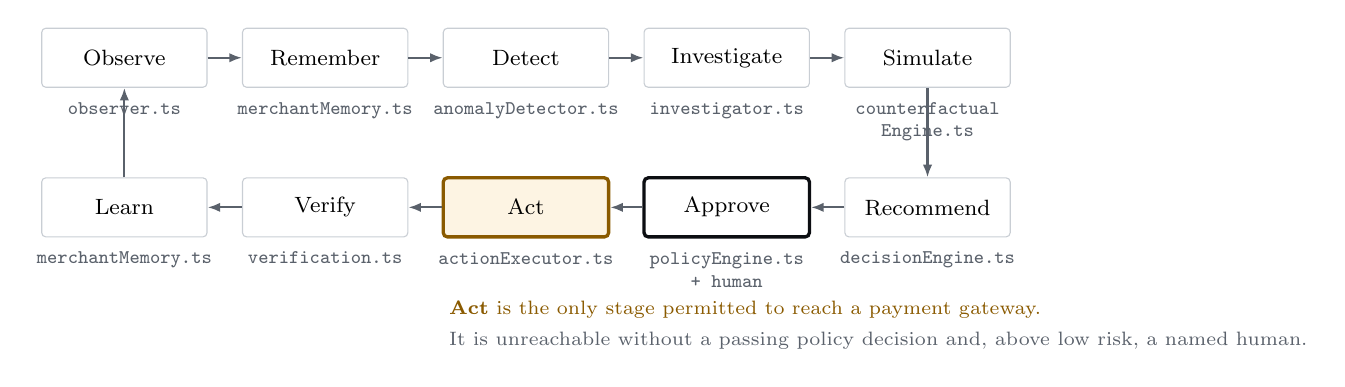
\begin{tikzpicture}[
  font=\footnotesize,
  stage/.style={
    draw=linegrey, fill=white, rounded corners=1.5pt,
    minimum width=21mm, minimum height=7.5mm, align=center, inner sep=1.5pt
  },
  gate/.style={stage, draw=amber, very thick, fill=amberbg},
  human/.style={stage, draw=ink, very thick},
  mod/.style={font=\scriptsize\ttfamily, text=inkmid, align=center},
  arr/.style={-{Latex[length=1.6mm]}, draw=inkmid, thick}
]

\def\dx{25.5mm}

\node[stage] (s1) at (0*\dx, 0) {Observe};
\node[stage] (s2) at (1*\dx, 0) {Remember};
\node[stage] (s3) at (2*\dx, 0) {Detect};
\node[stage] (s4) at (3*\dx, 0) {Investigate};
\node[stage] (s5) at (4*\dx, 0) {Simulate};

\node[stage] (s6) at (4*\dx, -19mm) {Recommend};
\node[human] (s7) at (3*\dx, -19mm) {Approve};
\node[gate]  (s8) at (2*\dx, -19mm) {Act};
\node[stage] (s9) at (1*\dx, -19mm) {Verify};
\node[stage] (s10) at (0*\dx, -19mm) {Learn};

\node[mod, below=0.6mm of s1]  {observer.ts};
\node[mod, below=0.6mm of s2]  {merchantMemory.ts};
\node[mod, below=0.6mm of s3]  {anomalyDetector.ts};
\node[mod, below=0.6mm of s4]  {investigator.ts};
\node[mod, below=0.6mm of s5]  {counterfactual\\Engine.ts};

\node[mod, below=0.6mm of s6]  {decisionEngine.ts};
\node[mod, below=0.6mm of s7]  {policyEngine.ts\\+ human};
\node[mod, below=0.6mm of s8]  {actionExecutor.ts};
\node[mod, below=0.6mm of s9]  {verification.ts};
\node[mod, below=0.6mm of s10] {merchantMemory.ts};

\draw[arr] (s1) -- (s2);
\draw[arr] (s2) -- (s3);
\draw[arr] (s3) -- (s4);
\draw[arr] (s4) -- (s5);
\draw[arr] (s5.south) -- ++(0,-4mm) -- (s6.north);
\draw[arr] (s6) -- (s7);
\draw[arr] (s7) -- (s8);
\draw[arr] (s8) -- (s9);
\draw[arr] (s9) -- (s10);
\draw[arr] (s10.north) -- ++(0,4mm) -- (s1.south);

\node[font=\scriptsize, text=amber, anchor=west] at ($(s8.south) + (-11mm,-9mm)$)
  {\textbf{Act} is the only stage permitted to reach a payment gateway.};
\node[font=\scriptsize, text=inkmid, anchor=west] at ($(s8.south) + (-11mm,-13mm)$)
  {It is unreachable without a passing policy decision and, above low risk, a named human.};

\end{tikzpicture}
}
  \caption{The ten-stage loop. Each stage is a module under \code{lib/}, not a
  service. \stage{Act} is the only stage with gateway access, and it is
  unreachable without a passing policy decision and, above low risk, a named
  human approval.}
  \label{fig:loop}
\end{figure*}

\subsection{Stage responsibilities}

\begin{description}[style=nextline, leftmargin=0pt]
  \item[\stage{Observe} --- \code{observer.ts}]
    Reduces the ledger to ten scalar signals (failure rate, success rate since
    onset, issuer share of failures, method mix, per-SKU refund rate, checkout
    conversion, settlement variance, settlement delay, overdue receivables,
    chargeback exposure), each with its window and sample size. It measures; it
    decides nothing.
  \item[\stage{Remember} --- \code{merchantMemory.ts}]
    Loads seven learned baselines from 42 days of history, each with a
    confidence, an observation count, a source and a plain-language statement of
    why the system believes it.
  \item[\stage{Detect} --- \code{anomalyDetector.ts}]
    Emits an anomaly where an observation has left its learned band \emph{by
    enough to matter financially}. Every anomaly carries an impact in rupees, a
    modelled recoverable amount, a confidence and an affected count.
  \item[\stage{Investigate} --- \code{investigator.ts}]
    Assembles evidence, segments the cohort, states a root cause with a
    mechanism, and --- importantly --- records the competing hypotheses it
    tested and why each was rejected.
  \item[\stage{Simulate} --- \code{counterfactualEngine.ts}]
    Scores every candidate response, including inaction, on the same three
    quantities (Section~\ref{sec:cf}).
  \item[\stage{Recommend} --- \code{decisionEngine.ts}]
    Converts the winning scenario into a \emph{bounded action plan}: an explicit
    cohort, a per-customer ceiling, an attempt ceiling, a risk rating and a named
    policy.
  \item[\stage{Approve} --- \code{policyEngine.ts} + UI]
    Deterministic rule evaluation, then a human where the policy demands one.
  \item[\stage{Act} --- \code{actionExecutor.ts}]
    The only module permitted to call a gateway. Runs in five observable stages.
  \item[\stage{Verify} --- \code{verification.ts}]
    Re-reads the outcome against the ledger and against the guardrails the action
    was approved under. A partial verdict is a legitimate result.
  \item[\stage{Learn} --- \code{merchantMemory.ts}]
    Baselines are recalibrated on verified outcomes; the recalibration itself is
    an audit event.
\end{description}

\subsection{State and determinism}

The read path is a pure function of a single seed (\code{DEMO\_SEED =
20260218}) and a fixed clock (\code{2026-02-18T16:45:00+05:30}).
\code{Math.random()} does not appear anywhere in the codebase; all randomness
comes from a seeded \code{mulberry32} generator. The dataset is built once per
process and cached on \code{globalThis}, so it survives module reloads and is
identical across processes, machines and deployments.

Write state --- which actions the operator approved, executed or rejected, and
the audit events those produced --- is held client-side behind a
\code{useSyncExternalStore}. This is not a shortcut: it keeps the server read
path referentially transparent, it survives a serverless cold start on Vercel
where a module-level mutation would not, and it makes \emph{Reset demo} exact
rather than approximate.

%==============================================================================
\section{Data model}
\label{sec:data}

Twenty-two entities span a ledger layer and an intelligence layer.
Figure~\ref{fig:er} shows the relationships; Table~\ref{tab:entities} lists the
entities with their role and cardinality in the seeded batch.

\begin{figure*}[t]
  \centering
  \resizebox{0.98\textwidth}{!}{% Entity relationships, ledger layer (left) and intelligence layer (right).
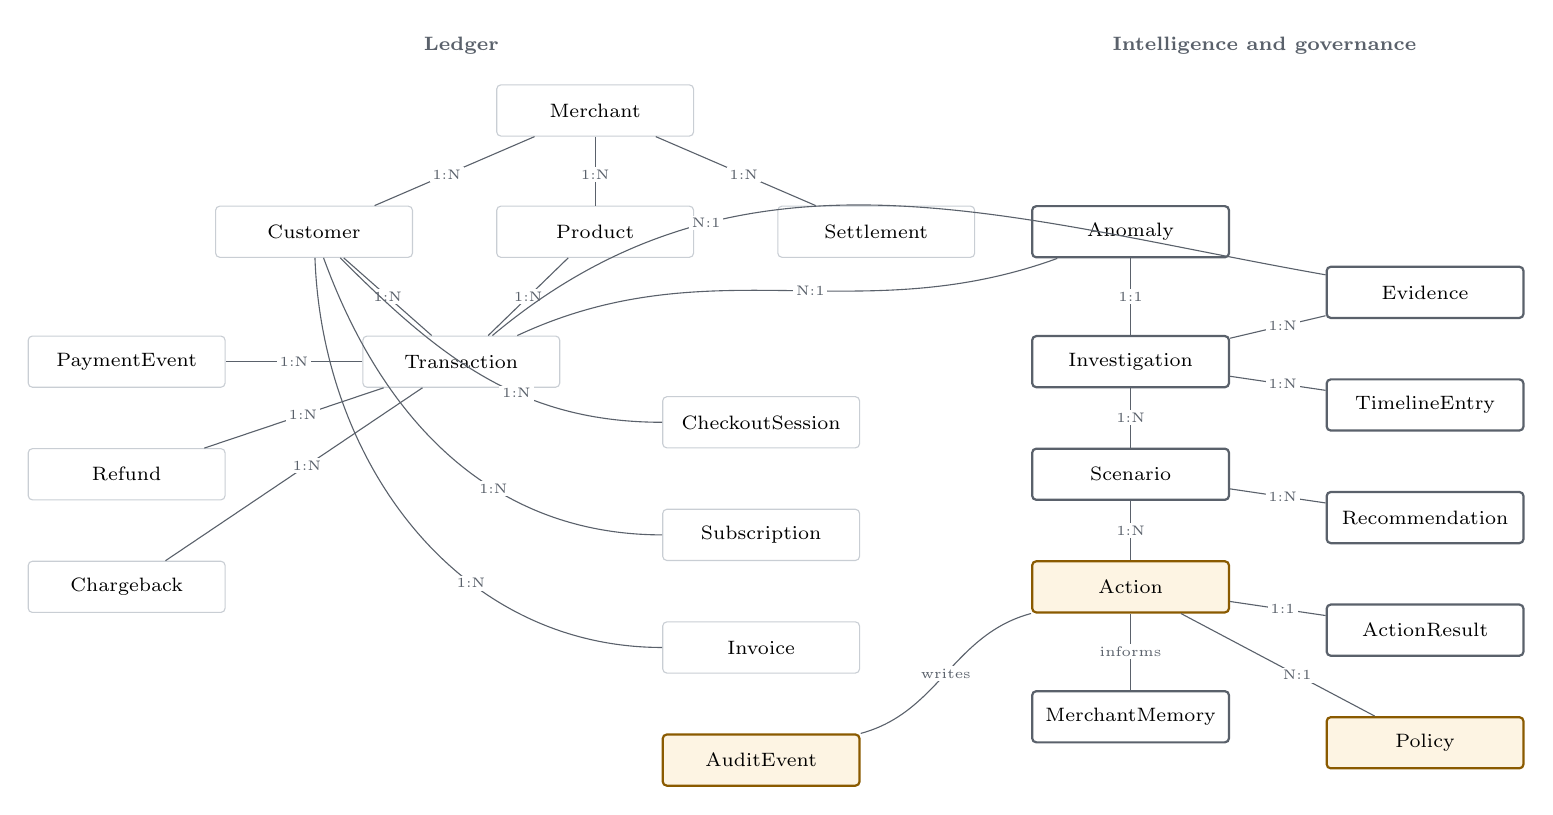
\begin{tikzpicture}[
  font=\scriptsize,
  ent/.style={draw=linegrey, fill=white, rounded corners=1.5pt,
              minimum width=25mm, minimum height=6.5mm, align=center, inner sep=2pt},
  led/.style={ent},
  intel/.style={ent, draw=inkmid, thick},
  gov/.style={ent, draw=amber, thick, fill=amberbg},
  rel/.style={draw=inkmid, thin},
  lbl/.style={font=\tiny, text=inkmid, fill=white, inner sep=1pt}
]

\def\cx{34mm}
\def\cy{11mm}

% ---- ledger layer -------------------------------------------------------
\node[led] (mer)  at (0, 0)                 {Merchant};
\node[led] (cus)  at (-1.05*\cx, -1.4*\cy)  {Customer};
\node[led] (pro)  at (0, -1.4*\cy)          {Product};
\node[led] (set)  at (1.05*\cx, -1.4*\cy)   {Settlement};
\node[led] (txn)  at (-0.5*\cx, -2.9*\cy)   {Transaction};
\node[led] (pev)  at (-1.75*\cx, -2.9*\cy)  {PaymentEvent};
\node[led] (ref)  at (-1.75*\cx, -4.2*\cy)  {Refund};
\node[led] (cbk)  at (-1.75*\cx, -5.5*\cy)  {Chargeback};
\node[led] (chk)  at (0.62*\cx, -3.6*\cy)   {CheckoutSession};
\node[led] (sub)  at (0.62*\cx, -4.9*\cy)   {Subscription};
\node[led] (inv)  at (0.62*\cx, -6.2*\cy)   {Invoice};

% ---- intelligence and governance layer ----------------------------------
\node[intel] (ano)  at (2.0*\cx, -1.4*\cy)  {Anomaly};
\node[intel] (ivg)  at (2.0*\cx, -2.9*\cy)  {Investigation};
\node[intel] (evd)  at (3.1*\cx, -2.1*\cy)  {Evidence};
\node[intel] (tml)  at (3.1*\cx, -3.4*\cy)  {TimelineEntry};
\node[intel] (scn)  at (2.0*\cx, -4.2*\cy)  {Scenario};
\node[intel] (rec)  at (3.1*\cx, -4.7*\cy)  {Recommendation};
\node[gov]   (act)  at (2.0*\cx, -5.5*\cy)  {Action};
\node[intel] (ares) at (3.1*\cx, -6.0*\cy)  {ActionResult};
\node[intel] (mem)  at (2.0*\cx, -7.0*\cy)  {MerchantMemory};
\node[gov]   (pcy)  at (3.1*\cx, -7.3*\cy)  {Policy};
\node[gov]   (aev)  at (0.62*\cx, -7.5*\cy) {AuditEvent};

% ---- ledger relations ---------------------------------------------------
\draw[rel] (mer) -- node[lbl,pos=0.55]{1:N} (cus);
\draw[rel] (mer) -- node[lbl,pos=0.55]{1:N} (pro);
\draw[rel] (mer) -- node[lbl,pos=0.55]{1:N} (set);
\draw[rel] (cus) -- node[lbl,pos=0.5]{1:N} (txn);
\draw[rel] (pro) -- node[lbl,pos=0.5]{1:N} (txn);
\draw[rel] (txn) -- node[lbl,pos=0.5]{1:N} (pev);
\draw[rel] (txn) -- node[lbl,pos=0.45]{1:N} (ref);
\draw[rel] (txn) -- node[lbl,pos=0.45]{1:N} (cbk);
\draw[rel] (cus) to[out=-45,in=180] node[lbl,pos=0.6]{1:N} (chk);
\draw[rel] (cus) to[out=-70,in=180] node[lbl,pos=0.62]{1:N} (sub);
\draw[rel] (cus) to[out=-88,in=180] node[lbl,pos=0.64]{1:N} (inv);

% ---- intelligence relations ---------------------------------------------
\draw[rel] (txn) to[out=25,in=200] node[lbl,pos=0.55]{N:1} (ano);
\draw[rel] (ano) -- node[lbl,pos=0.5]{1:1} (ivg);
\draw[rel] (ivg) -- node[lbl,pos=0.55]{1:N} (evd);
\draw[rel] (ivg) -- node[lbl,pos=0.55]{1:N} (tml);
\draw[rel] (ivg) -- node[lbl,pos=0.5]{1:N} (scn);
\draw[rel] (scn) -- node[lbl,pos=0.55]{1:N} (rec);
\draw[rel] (scn) -- node[lbl,pos=0.5]{1:N} (act);
\draw[rel] (act) -- node[lbl,pos=0.55]{1:1} (ares);
\draw[rel] (act) -- node[lbl,pos=0.6]{N:1} (pcy);
\draw[rel] (mem) -- node[lbl,pos=0.5]{informs} (act);
\draw[rel] (evd) to[out=170,in=40] node[lbl,pos=0.72]{N:1} (txn);
\draw[rel] (act) to[out=195,in=15] node[lbl,pos=0.5]{writes} (aev);

\node[font=\scriptsize\bfseries, text=inkmid] at (-0.5*\cx, 0.75*\cy) {Ledger};
\node[font=\scriptsize\bfseries, text=inkmid] at (2.5*\cx, 0.75*\cy) {Intelligence and governance};

\end{tikzpicture}
}
  \caption{Entity relationships. The ledger layer (left) is what a payment
  platform already has. The intelligence and governance layer (right) is what
  turns it into decisions, and every entity in it is traceable back to
  transactions.}
  \label{fig:er}
\end{figure*}

\begin{table}[t]
\centering
\small
\begin{tabular}{@{}l r l@{}}
\toprule
\textbf{Entity} & \textbf{Rows} & \textbf{Role} \\
\midrule
Merchant          & 1      & Tenant root \\
Customer          & 3{,}200 & Repeat-purchase signal \\
Product           & 8      & Per-SKU refund analysis \\
Transaction       & 10{,}000 & The ledger \\
PaymentEvent      & derived & Lifecycle per transaction \\
Refund            & 333    & Refund-spike detection \\
Chargeback        & 9      & Dispute exposure \\
Settlement        & 14     & Reconciliation \\
CheckoutSession   & 742    & Funnel drop-off \\
Subscription      & 240    & Recurring failure risk \\
Invoice           & 118    & Receivables ageing \\
\midrule
Anomaly           & 7      & Detection output \\
Investigation     & 4      & Evidence-backed case \\
Evidence          & 10--12 & Traceable support \\
TimelineEntry     & 4--6   & What ran, when \\
Scenario          & 3/case & Priced alternatives \\
Recommendation    & 1/case & Selected scenario \\
Action            & 9      & Bounded plan \\
ActionResult      & 1/exec & Outcome + verification \\
AuditEvent        & 31+    & The chain of record \\
MerchantMemory    & 7      & Learned baselines \\
Policy            & 1      & \code{RECOVERY\_V2 · 2.3} \\
\bottomrule
\end{tabular}
\caption{Entities and their cardinality in the seeded batch. Row counts are the
values the running application reports at \code{/api/diagnostics}.}
\label{tab:entities}
\end{table}

The schema is expressed canonically in \code{prisma/schema.prisma}, and
\code{lib/types.ts} mirrors it field for field. The demo materialises it in
memory rather than in Postgres --- a deliberate choice, since requiring a
database to see the product would defeat the point --- but the two are the same
shape, so moving to a persistent deployment is a repository-layer change and not
a UI change.

Two fields on \code{Transaction} deserve mention because the rest of the system
leans on them. \code{anomalyId} attributes a transaction to a detected anomaly,
which is what makes ``1{,}284 affected payments'' a query rather than a claim.
\code{recoveryProbability} is a per-transaction model output, present only on
failures, and is the basis of every ``recoverable'' figure in the product.

%==============================================================================
\section{Detection and investigation}
\label{sec:detect}

\subsection{The synthetic batch}

The dataset covers 24 hours ending at the fixed clock and is \emph{constructed}
to its targets rather than sampled and hoped over. Amounts are scaled so that
cohort totals are exact (\code{scaleToTotal}, and \code{scaleToTotalCapped}
where a policy ceiling must hold for every member by construction). Segment
shares are struck by even stride rather than Bernoulli sampling, because
Bernoulli sampling leaves an 87\% target sitting at 84\% and a report should not
have to round.

The batch is shaped in three windows:

\begin{table}[h]
\centering
\small
\begin{tabular}{@{}l r r r@{}}
\toprule
\textbf{Window} & \textbf{Attempts} & \textbf{Failures} & \textbf{Success} \\
\midrule
00:00--09:12 (pre)   & 2{,}382 & 52    & 97.8\% \\
09:12--16:45 (event) & 7{,}618 & 1{,}415 & 81.4\% \\
\quad of which 14:30--16:10 & 1{,}099 & 494 & 55.1\% \\
\midrule
Day total            & 10{,}000 & 1{,}467 & 85.3\% \\
\bottomrule
\end{tabular}
\end{table}

Captured value is \rs{}18{,}42{,}000 across 8{,}533 payments, an average order
value of \rs{}216. The affected cohort averages \rs{}375 --- a 1.7$\times$ skew
that the investigation surfaces as evidence in its own right, since
higher-value collect requests failing first is consistent with issuer-side risk
checks queueing behind a saturated service.

\subsection{The five required anomaly classes}

\begin{enumerate}
  \item \textbf{UPI payment degradation} (\code{inv\_1042}, critical) ---
    \rs{}4.82L across 1{,}284 payments, 91\% confidence.
  \item \textbf{Refund spike on one SKU} (\code{inv\_1043}, watch) --- Aurora
    Buds Pro, 3.7\% $\rightarrow$ 8.9\%, \rs{}1.10L of excess refund value over
    nine days, 88\% confidence.
  \item \textbf{Checkout conversion drop} (\code{inv\_1044}, watch) --- 93.8\%
    $\rightarrow$ 91.8\%, 61 abandoned sessions, \rs{}72K, 76\% confidence.
  \item \textbf{Settlement discrepancy} (\code{inv\_1045}, watch) --- \rs{}38K
    unreconciled on 1 of 14 cycles, 84\% confidence.
  \item \textbf{Recoverable failed payments} (opportunity) --- 184 high-intent
    customers, \rs{}1.92L exposure, \rs{}1.26L modelled recoverable.
\end{enumerate}

Two further findings --- receivables ageing (\rs{}82K across 27 invoices) and
chargeback exposure (\rs{}58K across 9 disputes) --- complete the \rs{}8.42L
risk rollup. The rollup is a sum over the anomaly ledger, and the
\emph{recoverable failed payments} entry is explicitly excluded from it because
it is a view onto the UPI cohort rather than a separate exposure. Double-counting
exposure is the easiest way for a product like this to lie, so the exclusion is
enforced in code (\code{DERIVED\_ANOMALIES}) rather than by convention.

\subsection{From evidence to root cause}

The investigation workspace is deliberately not a chat interface. It assembles
ten evidence items for the UPI case, each weighted:

\begin{itemize}
  \item six \emph{transaction} items --- the highest-value failures, each opening
    a drawer with the full payment-event trail, customer history and error code;
  \item three \emph{aggregate} and \emph{timeseries} items --- issuer
    concentration, method/device cut, and the 20-minute success-rate series;
  \item one \emph{comparison} item --- the order-value skew.
\end{itemize}

The root cause is stated with a mechanism, not just a label: collect requests to
the issuer are timing out before customer approval, which the gateway reports as
a timeout rather than a decline. It is supported by a two-bar comparison of the
issuer's baseline failure share (21\%) against its incident share (87\%).

What makes this an investigation rather than an assertion is the record of
\emph{rejected} hypotheses:

\begin{table}[h]
\centering
\small
\begin{tabular}{@{}p{0.31\columnwidth} p{0.57\columnwidth}@{}}
\toprule
\textbf{Hypothesis} & \textbf{Rejected because} \\
\midrule
Merchant-side checkout regression & Card success is 97.6\% and netbanking 97.1\% today; a checkout regression would not spare two rails \\
Customer balance or auth failures & 86\% of affected error codes are timeouts or gateway errors; declines are flat \\
Traffic shift toward UPI & UPI's share of attempts is 61\% against a 62\% baseline \\
Android release regression & Android carries 88\% of failures but 58\% of all traffic; iOS payments on the same issuer fail at the same elevated rate \\
\bottomrule
\end{tabular}
\caption{Alternative hypotheses tested and dismissed for \code{inv\_1042}. A
confidence score without this table is a number without a method.}
\end{table}

Confidence is reported at two levels and they are not the same number: 91\% on
the root cause, 82\% on the recovery estimate. Conflating them would overstate
how much is known about the money.

%==============================================================================
\section{The counterfactual engine}
\label{sec:cf}

This is the component that separates a decision system from an alerting system,
and it is a safety property before it is a feature.

Every candidate response, \emph{including doing nothing}, is scored on the same
three quantities:

\[
\begin{aligned}
R &= V_{\text{risk}} \times r_{\text{conv}} &&\text{expected recovery}\\
C &= c_{\text{unit}} \times n_{\text{attempts}} &&\text{expected cost}\\
B &= R - C &&\text{net expected benefit}
\end{aligned}
\]

with inaction scored as a loss, $L = V_{\text{risk}} \times r_{\text{churn}}$,
so that $B_{\text{do nothing}} = -L$. Table~\ref{tab:scenarios} gives the scored
alternatives for the UPI case, where $V_{\text{risk}}$ is \rs{}4{,}82{,}000.

\begin{table}[h]
\centering
\small
\begin{tabular}{@{}l r r r@{}}
\toprule
\textbf{Scenario} & \textbf{Recovery} & \textbf{Cost} & \textbf{Net} \\
\midrule
A. Do nothing            & ---        & ---      & $-$\rs{}2.10L \\
B. Retry failed payments & \rs{}1.70L & \rs{}12K & \rs{}1.58L \\
C. Alternate rail offer  & \rs{}2.40L & \rs{}28K & \textbf{\rs{}2.12L} \\
\bottomrule
\end{tabular}
\caption{Counterfactuals for \code{inv\_1042}. Conversion is modelled at 35.3\%
for a retry, because it lands on the same degraded rail, and 49.8\% for the
alternate rail. Retry cost is \rs{}4.67 per attempt over two attempts across
1{,}284 payments; outreach cost is \rs{}21.80 per contacted customer. Scenario C
wins on net expected benefit and is recommended.}
\label{tab:scenarios}
\end{table}

Three properties matter more than the arithmetic.

\textbf{Inaction is priced.} A merchant who declines every recommendation should
still be told what that decision costs. Presenting a loss of \rs{}2.10L next to
a gain of \rs{}2.12L turns ``do nothing'' from a default into a choice.

\textbf{The comparison is made before the recommendation, not after.} The
decision engine does not generate a plan and then justify it; it takes the
argmax of $B$ over the scored set. The recommendation text is derived from that
ranking, which is why it can cite the runner-up (``\rs{}2.12L net against
\rs{}1.58L for a retry on the same degraded rail'').

\textbf{Each scenario states its assumptions.} Conversion rates, unit costs and
the policy ceilings that bound the scenario are shown on the card. A merchant
who disagrees with the 49.8\% conversion assumption can see it and say so, which
is not possible when the model emits only a conclusion.

The recommended scenario is then \emph{narrowed} into an action. Scenario C
covers all 1{,}284 payments; the action targets only the 184 high-intent
customers --- one failed attempt each, all priced under the policy ceiling ---
for \rs{}1.42L of expected recovery. A first tranche that a human can inspect is
worth more than a complete plan that a human cannot.

%==============================================================================
\section{Decision safety architecture}
\label{sec:safety}

\begin{figure*}[t]
  \centering
  \resizebox{0.86\textwidth}{!}{% Decision-safety pipeline: from model output to audited outcome.
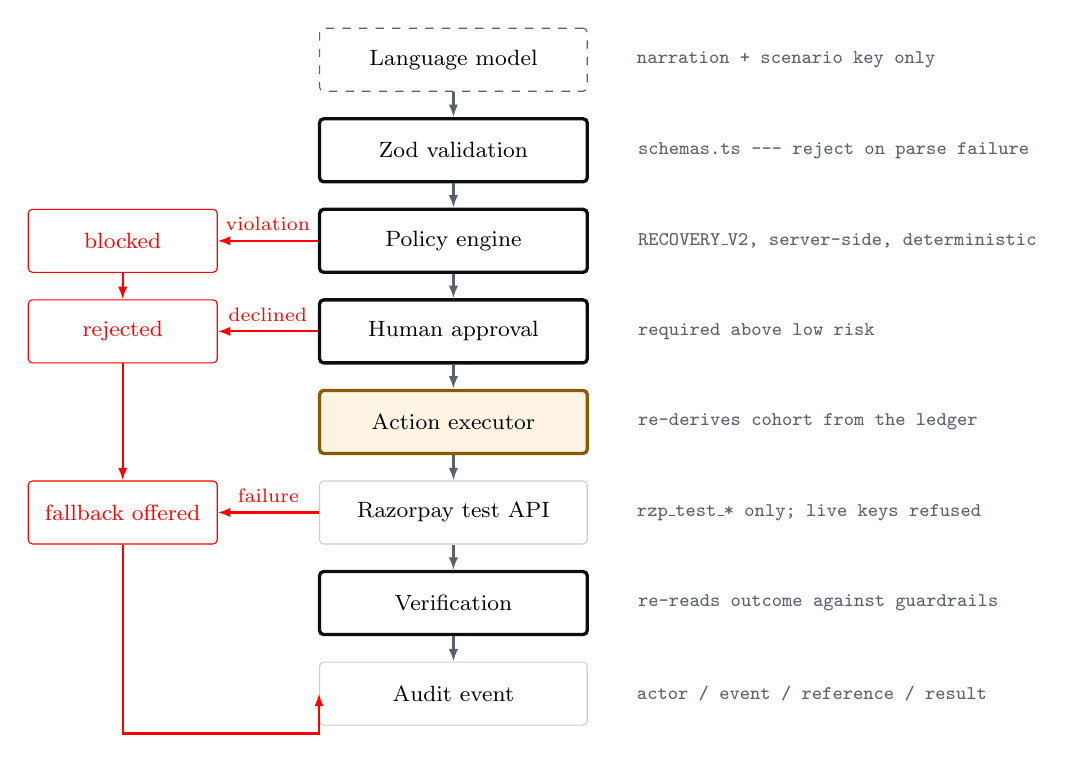
\begin{tikzpicture}[
  font=\footnotesize,
  box/.style={draw=linegrey, fill=white, rounded corners=1.5pt,
              minimum width=34mm, minimum height=8mm, align=center, inner sep=2pt},
  soft/.style={box, draw=inkmid, dashed},
  hard/.style={box, draw=ink, very thick},
  gate/.style={box, draw=amber, very thick, fill=amberbg},
  note/.style={font=\scriptsize\ttfamily, text=inkmid, anchor=west},
  arr/.style={-{Latex[length=1.6mm]}, draw=inkmid, thick}
]

\def\dy{11.5mm}

\node[soft] (llm)    at (0, 0)        {Language model};
\node[hard] (zod)    at (0, -1*\dy)   {Zod validation};
\node[hard] (pol)    at (0, -2*\dy)   {Policy engine};
\node[hard] (hum)    at (0, -3*\dy)   {Human approval};
\node[gate] (exec)   at (0, -4*\dy)   {Action executor};
\node[box]  (rzp)    at (0, -5*\dy)   {Razorpay test API};
\node[hard] (ver)    at (0, -6*\dy)   {Verification};
\node[box]  (aud)    at (0, -7*\dy)   {Audit event};

\foreach \a/\b in {llm/zod, zod/pol, pol/hum, hum/exec, exec/rzp, rzp/ver, ver/aud}
  \draw[arr] (\a) -- (\b);

\node[note] at ($(llm.east)  + (5mm,0)$) {narration + scenario key only};
\node[note] at ($(zod.east)  + (5mm,0)$) {schemas.ts --- reject on parse failure};
\node[note] at ($(pol.east)  + (5mm,0)$) {RECOVERY\_V2, server-side, deterministic};
\node[note] at ($(hum.east)  + (5mm,0)$) {required above low risk};
\node[note] at ($(exec.east) + (5mm,0)$) {re-derives cohort from the ledger};
\node[note] at ($(rzp.east)  + (5mm,0)$) {rzp\_test\_* only; live keys refused};
\node[note] at ($(ver.east)  + (5mm,0)$) {re-reads outcome against guardrails};
\node[note] at ($(aud.east)  + (5mm,0)$) {actor / event / reference / result};

% Blocked branches
\node[box, draw=red, text=red, minimum width=24mm] (blk)
  at (-42mm, -2*\dy) {blocked};
\draw[arr, draw=red] (pol.west) -- node[above, font=\scriptsize, text=red] {violation} (blk.east);

\node[box, draw=red, text=red, minimum width=24mm] (rej)
  at (-42mm, -3*\dy) {rejected};
\draw[arr, draw=red] (hum.west) -- node[above, font=\scriptsize, text=red] {declined} (rej.east);

\node[box, draw=red, text=red, minimum width=24mm] (fbk)
  at (-42mm, -5*\dy) {fallback offered};
\draw[arr, draw=red] (rzp.west) -- node[above, font=\scriptsize, text=red] {failure} (fbk.east);

\draw[arr, draw=red] (blk.south) -- (rej.north);
\draw[arr, draw=red] (rej.south) -- ++(0,-\dy) -- (fbk.north);
\draw[arr, draw=red] (fbk.south) -- ++(0,-24mm) -| (aud.west);

\end{tikzpicture}
}
  \caption{The mandatory pipeline. Red branches are terminal outcomes that are
  themselves audited: a policy block, a human rejection and a gateway failure all
  end in an audit event rather than in silence.}
  \label{fig:pipeline}
\end{figure*}

The single most important design decision in this product is stated negatively:
\textbf{the language model cannot execute a financial action}. Not ``is
instructed not to'' --- cannot. The boundary is structural, and it is enforced in
four places.

\paragraph{1. The model's output surface is a closed set.}
The only structured output a model may produce is a \code{scenarioKey} drawn
from the three scenarios the counterfactual engine already scored, plus prose.
The Zod schema (\code{llmRecommendationSchema}) admits
\code{do\_nothing $\mid$ retry $\mid$ alternate\_method}, a headline, a reason
and a confidence. There is no field for an endpoint, an amount, a cohort, a
customer list or a policy name. A model that emits one is rejected at parse time
and the deterministic engine's choice stands.

\paragraph{2. The executor takes an identifier, not an instruction.}
\code{runStage(actionId, stage, constraints)} looks the plan up server-side and
re-derives the cohort from the ledger. The HTTP body carries a stage name and,
optionally, constraints. Nothing else crosses the boundary.

\paragraph{3. Constraints can only narrow.}
An operator may reduce a cohort or lower a ceiling from the UI. The executor
applies \code{Math.min(plan, request)} on both, so a client that requests a
larger cohort or a higher ceiling \emph{tightens} the action rather than widening
it. Attempting to widen is not an error condition to be handled; it is
structurally impossible to express.

\paragraph{4. Credentials refuse live mode.}
\code{assertTestMode} rejects any key that does not begin with
\code{rzp\_test\_}, and it is called on the authorisation header path, not only
at configuration time. There is no code path in the repository that can
authenticate against live mode.

To this we add a fifth property that is not about the model at all: the product
never claims an external call that did not happen. Without credentials, gateway
responses are labelled \code{MOCK\_*} and their messages say, in the response
body that the UI renders, that no request was sent to Razorpay. Actions that need
no gateway --- a refund hold, a checkout reordering, a reconciliation filing ---
report ``Gateway: not required for this action class'' rather than manufacturing
a call.

%==============================================================================
\section{Policy engine}
\label{sec:policy}

The policy engine is a pure function of an action plan and a policy. It contains
no model output, no probability and no I/O. It runs server-side on \emph{every}
stage of an execution, not once at approval, so an action cannot become
non-compliant part-way through a run.

\begin{table}[h]
\centering
\small
\begin{tabular}{@{}>{\scriptsize\ttfamily}l l p{0.42\columnwidth}@{}}
\toprule
\textrm{\textbf{Rule}} & \textbf{Value} & \textbf{Rationale} \\
\midrule
MAX\_AUTO\_ACTION\_AMOUNT & \rs{}5{,}000 & Bounds the worst case of a single mis-targeted action to a sum the merchant can absorb and reverse \\
MAX\_RETRY\_ATTEMPTS & 2 & Repeated retries on a degraded rail add cost, irritate customers and can trip issuer risk rules; two attempts capture nearly all recoverable value \\
MAX\_DISCOUNT\_PERCENT & 10\% & Beyond this, recovery costs more than the order earns \\
HIGH\_RISK\_REQUIRES\_APPROVAL & true & Customer-contacting and money-moving actions carry reputational consequences the model cannot price \\
MAX\_CUSTOMERS\_PER\_ACTION & 500 & Caps how many customers one mistake reaches before a human sees a result \\
TEST\_MODE\_ONLY & true & No live-money credential is loadable here \\
\bottomrule
\end{tabular}
\caption{\code{RECOVERY\_V2 · 2.3}. Each threshold answers ``what is the worst
outcome if this action is wrong?'', not ``what is the best outcome if it is
right?''}
\label{tab:policy}
\end{table}

The ceilings are visibly load-bearing rather than decorative. The six largest
failures in the incident total \rs{}59{,}880 and every one of them exceeds
\rs{}5{,}000, so no automated action may touch them; they are shown on the action
page under \emph{Held for manual approval} with their transaction identifiers. The
historical action ledger contains \code{act\_2026}, a 640-customer retry that was
blocked before approval by \code{MAX\_CUSTOMERS\_PER\_ACTION} and re-scoped to
500, and \code{act\_2028}, a 15\% blanket discount rejected by the merchant. Of
143 actions executed across the batch, 12 were blocked by policy and 37 required
a human approval.

%==============================================================================
\section{Graceful failure handling}
\label{sec:failure}

An always-succeeds demo proves nothing about production-readiness. The
interesting question about an agent is not what it does when the world
cooperates. The system therefore ships a deterministic failure and treats it as a
first-class path.

\code{act\_2040}, ``Retry failed UPI payments'', targets the same 184-customer
cohort as the recommended action. It has already spent one of its two automatic
attempts during the incident --- which is visible in the payment-event trail of
every affected transaction --- so it is \emph{allowed} to run, and it does.

\begin{enumerate}
  \item \stage{Prepare}. Cohort re-derived from the ledger: 184 targets,
    \rs{}1{,}92{,}000 exposure.
  \item \stage{Policy}. Five of five rules pass. \code{MAX\_RETRY\_ATTEMPTS}
    reports ``1 of 2 attempts used'' --- the action is compliant.
  \item \stage{Eligibility}. 184 of 184 eligible; 6 larger failures worth
    \rs{}59{,}880 remain outside automation.
  \item \stage{Gateway}. A recovery order is created, then queried for captured
    payments. None is found inside the attempt window. This is an
    \emph{observed negative result}, not a fabricated one: in Live Test Mode it
    is a real \code{GET /v1/orders/:id/payments} returning an empty
    \code{items} array.
  \item \textbf{Policy re-evaluation.} The executor re-runs the policy with
    \code{attemptsUsed + 1}. \code{MAX\_RETRY\_ATTEMPTS} now fails. Further
    retries are halted.
  \item \stage{Verify} is never reached. The run is terminal.
\end{enumerate}

The UI does not crash, does not spin and does not show a stack trace. It shows:

\begin{quote}\small
\textbf{Action could not be completed}\\[2pt]
\textbf{Reason.} Temporary payment failure.\\
\textbf{Policy.} Retry ceiling reached --- 2 of 2 attempts already spent on this
cohort.\\
\textbf{AI response.} ``I will not repeatedly retry this payment. The configured
policy limit has been reached, and a further attempt against the same degraded
rail would add cost without adding expected recovery. An alternate recovery
workflow is available.''
\end{quote}

and a single button, \emph{Review alternative}, which routes to
\code{act\_2041}. Three audit events are written: the gateway call, the
\code{TEMPORARY\_PAYMENT\_FAILURE}, and the policy activation of the fallback.
The failure is not a dead end and it is not hidden; it is a transition with a
record.

The fallback then completes. Against a modelled \rs{}1{,}42{,}080, the executed
alternate-rail action recovers \rs{}1{,}41{,}175 across 130 of 184 customers, and
verification passes all five checks. Reporting a realised figure that differs
from the model, rather than echoing the estimate back, is the point: a system
that always ``recovers exactly what it predicted'' is not measuring anything.

%==============================================================================
\section{Audit trail design}
\label{sec:audit}

Every event carries the same tuple:

\begin{center}\small
\code{(at, actor, event, refType, refId, result, detail)}
\end{center}

with \code{actor} $\in$ \{\code{ai}, \code{merchant}, \code{api}, \code{policy},
\code{system}\} and \code{result} $\in$ \{\code{ok}, \code{failed},
\code{blocked}, \code{info}\}. The stream is filterable by actor and by failure,
and events generated during the current session are visually distinguished from
the seeded history.

The design goal is reconstruction without context. An auditor reading only the
audit trail can answer: what was detected, and on what evidence; who or what
opened the investigation; what root cause was concluded; what was recommended and
why it was held for approval; who approved it; which policy passed and when;
which endpoint was called and with what response; what failed; which rule halted
it; what was offered instead; what was recovered; and whether the result was
verified. Table~\ref{tab:audit} is that chain for the demo run.

\begin{table*}[t]
\centering
\small
\begin{tabular}{@{}l l l l l@{}}
\toprule
\textbf{Time (IST)} & \textbf{Actor} & \textbf{Event} & \textbf{Reference} & \textbf{Result} \\
\midrule
14:32:11 & ai       & AI detected payment anomaly       & \code{anm\_upi\_degradation} & info \\
14:33:04 & ai       & Investigation created             & \code{inv\_1042}   & ok \\
14:34:12 & ai       & Payment methods segmented         & \code{inv\_1042}   & info \\
14:35:01 & ai       & Root cause identified             & \code{inv\_1042}   & ok \\
14:36:20 & ai       & Revenue impact calculated         & \code{inv\_1042}   & info \\
14:36:48 & ai       & Counterfactuals scored            & \code{inv\_1042}   & info \\
14:37:02 & ai       & Recovery recommendation generated & \code{act\_2041}   & ok \\
14:37:03 & policy   & Approval requirement applied      & \code{RECOVERY\_V2} & blocked \\
16:45:30 & merchant & Action approved                   & \code{act\_2040}   & ok \\
16:45:33 & policy   & Policy validation passed          & \code{RECOVERY\_V2} & ok \\
16:45:36 & system   & Transaction eligibility checked   & \code{act\_2040}   & ok \\
16:45:41 & api      & Gateway called                    & \code{act\_2040}   & ok \\
16:45:41 & api      & \textbf{Payment retry failed}     & \code{act\_2040}   & \textbf{failed} \\
16:45:42 & policy   & \textbf{Fallback policy activated}& \code{RECOVERY\_V2} & \textbf{blocked} \\
16:47:00 & merchant & Action approved                   & \code{act\_2041}   & ok \\
16:47:11 & api      & Recovery offers dispatched        & \code{act\_2041}   & ok \\
16:47:27 & ai       & Result verified                   & \code{act\_2041}   & ok \\
\bottomrule
\end{tabular}
\caption{The demo chain end to end, as rendered at \code{/audit}. Rows above
16:45 are produced by the detection pipeline before any operator input; rows from
16:45 are produced by the executor during the session. The two bold rows are the
failure and the policy response to it.}
\label{tab:audit}
\end{table*}

Seeded history contributes a second complete chain from 12 February --- including
its own partial failure, fallback and post-recovery memory update --- so the
audit view is informative before a presenter touches anything.

%==============================================================================
\section{Merchant memory}
\label{sec:memory}

Seven baselines are learned from 42 days of history. Each carries a value, a
confidence, an observation count, a source, and a written explanation of why the
system believes it (Table~\ref{tab:memory}).

\begin{table}[h]
\centering
\small
\begin{tabular}{@{}l l l l@{}}
\toprule
\textbf{Baseline} & \textbf{Normal} & \textbf{Current} & \textbf{Status} \\
\midrule
Payment failure rate   & 2.1\%   & 14.7\%  & Unusual \\
Issuer concentration   & 21\%    & 87\%    & Unusual \\
UPI mix                & 62\%    & 61\%    & Normal \\
Refund rate (SKU-2481) & 3.7\%   & 8.9\%   & Unusual \\
Sunday revenue         & \rs{}7--9L & \rs{}8.2L & Normal \\
Settlement timing      & 1.3 d   & 1.4 d   & Normal \\
Checkout conversion    & 93.8\%  & 91.8\%  & Drifting \\
\bottomrule
\end{tabular}
\caption{Learned baselines. The \emph{Normal} rows are as important as the
unusual ones: they are what stops the detector raising an anomaly every Sunday
morning.}
\label{tab:memory}
\end{table}

Memory does three jobs. It \textbf{contextualises}: 8.9\% is meaningless in
isolation and unambiguous against a 3.7\% baseline held for 33 consecutive days.
It \textbf{suppresses}: Sunday revenue at a third of a weekday is structural for
this merchant, and encoding that prevents a weekly false positive. And it
\textbf{discriminates}: because UPI's share of \emph{attempts} is unchanged at
61\% while UPI \emph{fulfilment} has collapsed, the investigation can rule out a
customer-behaviour explanation and say so in the summary.

Baselines are recalibrated on verified outcomes. The 12 February recovery closed
with ``Recovery model recalibrated on 96 new observations'', written to the audit
trail --- learning is an auditable event, not an invisible drift.

%==============================================================================
\section{Results}
\label{sec:results}

Table~\ref{tab:results} reports the seeded batch. These are the figures the
running application computes; \code{GET /api/diagnostics} returns them live.

\begin{table}[h]
\centering
\small
\begin{tabular}{@{}l r@{}}
\toprule
\textbf{Measure} & \textbf{Value} \\
\midrule
Transactions analysed        & 10{,}000 \\
\quad captured / failed      & 8{,}533 / 1{,}467 \\
Captured value               & \rs{}18{,}42{,}000 \\
Average order value          & \rs{}216 \\
\midrule
Anomalies detected           & 37 \\
Investigations run           & 29 \\
Revenue at risk              & \rs{}8.42L \\
Potential recovery           & \rs{}5.17L \\
Actual recovered             & \rs{}3.84L \\
\midrule
Actions executed             & 143 \\
Actions blocked by policy    & 12 \\
Human approvals              & 37 \\
\midrule
\multicolumn{2}{@{}l}{\emph{Flagship case} \code{inv\_1042}} \\
Affected payments            & 1{,}284 \\
Revenue at risk              & \rs{}4{,}82{,}000 \\
Modelled recoverable         & \rs{}3{,}14{,}000 (65.2\%) \\
Success rate, pre / event    & 97.8\% / 81.4\% \\
Acute-window trough          & 55.1\% \\
Issuer failure share         & 21\% $\rightarrow$ 87\% (4.1$\times$) \\
High-intent cohort           & 184 / \rs{}1{,}92{,}000 \\
Held above policy ceiling    & 6 / \rs{}59{,}880 \\
Executed recovery            & \rs{}1{,}41{,}175 (130/184) \\
\quad against modelled       & \rs{}1{,}42{,}080 \\
\bottomrule
\end{tabular}
\caption{The seeded batch. All values are computed from the generated ledger,
not asserted; the generator is constructed to hit its targets exactly so that a
presenter sees the same numbers on every run.}
\label{tab:results}
\end{table}

The batch is a synthetic test environment and the report labels it as such
everywhere it appears. What the numbers demonstrate is internal consistency: the
\rs{}8.42L rollup is the sum of the anomaly ledger; the \rs{}4.82L is the sum of
1{,}284 transaction amounts; the \rs{}3.14L is the amount-weighted expectation
$\sum_i a_i p_i$ over those transactions; and the \rs{}1{,}41{,}175 realised
figure is the sum of the amounts of the 130 cohort members whose deterministic
draw fell below their uplifted recovery probability. No displayed figure is a
constant typed into a component.

%==============================================================================
\section{UI and UX design rationale}

The visual direction --- restrained neutral surfaces, hairline borders, a single
blue accent used sparingly, tabular figures throughout, monospace reserved for
identifiers and timestamps, high information density --- is not a style
preference. It follows from two requirements.

\textbf{Trustworthiness.} This product asks a merchant to approve an action that
contacts 184 of their customers. Interfaces that signal excitement --- gradients,
glow, oversized numbers, animated emphasis --- are precisely wrong for that
request. The design borrows the register of infrastructure documentation and
trading terminals because those are the interfaces people trust with
consequential decisions.

\textbf{Legibility of comparison.} Almost every screen is a comparison: observed
against baseline, scenario against scenario, realised against modelled. Density
serves that directly --- the counterfactual cards are readable side by side
without scrolling, the memory grid shows seven baselines at once, and the audit
table puts actor, event, reference and result on one line. Whitespace is spent on
separating comparisons, not on decorating them.

Concrete consequences: monospace for every identifier (\code{TXN\_82931},
\code{act\_2041}, \code{UTR6704666335}) so they are recognisable as machine
values; tabular figures so columns of money align; a two-pixel status rule at the
top of severity cards instead of a coloured background; animation confined to
execution progression and status transitions, where it carries meaning. Loading
states are skeletons of the eventual layout; error states name what could not be
read (``Unable to retrieve this transaction'') and offer a retry; no error
surface renders a stack trace.

%==============================================================================
\section{Tech stack and deployment}

Next.js 16 (App Router), React 19, TypeScript in strict mode, Tailwind CSS,
Recharts for the time-series and volume charts, hand-drawn SVG for sparklines,
Lucide for iconography, Zod for validation. Server Components read the domain
modules directly; Route Handlers cover the interactive paths; \code{server-only}
guards the gateway client and the executor at the module level so a client import
is a build error rather than a security incident.

The whole thing deploys with \code{vercel} or a GitHub import. There is no
Python, no FastAPI, no Docker, no Redis, no worker and no second deployment
target. Every route handler is a serverless function and every page is
server-rendered on demand.

Every environment variable is optional. With an empty environment the application
runs in full Demo Mode: deterministic data, deterministic detection and scoring,
a labelled local gateway adapter. Supplying a Razorpay test key pair switches the
badge to \emph{Live Test Mode} and makes the executor issue real calls against
the test environment. Supplying a model key switches the investigation summary
from the built-in deterministic text to model-written prose; nothing else
changes, because nothing else is allowed to depend on the model.

That property is a judgeability argument as much as an engineering one. A judge
with no keys, no database and a slow network still sees the complete product, and
can tell at a glance which mode it is in, because the badge says so on every
screen.

%==============================================================================
\section{Limitations and future work}

We are explicit about the boundary between what is built and what a live-money
deployment would require.

\textbf{Synthetic data.} Every figure describes a generated ledger. No real
merchant or customer data is present. A production deployment would read from the
merchant's own transaction and settlement records through the platform APIs.

\textbf{Recovery is modelled, not collected.} In Demo Mode ``recovered'' is a
deterministic outcome over the seeded cohort. In Live Test Mode the API calls are
real but create test-mode order objects; the recovery value is still modelled,
and the result message says so. Actually moving money would require payment
links, customer consent flows and reconciliation against real captures.

\textbf{The recovery model is calibrated, not trained.} Per-transaction
probabilities are drawn from a bounded distribution and normalised so the
amount-weighted mean matches a target. A production version would fit on the
merchant's own historical recovery outcomes, report a prediction interval rather
than a point estimate, and be re-fit on every verified action.

\textbf{Detection is baseline comparison.} Thresholds against learned bands, not
statistical process control or changepoint detection. This is deliberate for a
demo where determinism outranks sophistication, but a production detector would
want CUSUM or Bayesian changepoint methods with explicit false-positive budgets.

\textbf{Persistence and multi-tenancy.} Session state is per-browser and the
ledger is per-process. Production requires the Prisma schema against Postgres,
tenant isolation, and an append-only audit store with retention guarantees ---
an audit trail that can be edited is not an audit trail.

\textbf{Approval identity.} The demo records ``merchant'' as the approving actor.
A real deployment needs authenticated users, role-based authority limits (who may
approve above which value), and non-repudiation on the approval record.

\textbf{Adversarial robustness.} We constrain what the model can express, but we
have not adversarially tested prompt injection through merchant-controlled data
such as product names or refund reasons. The structural constraint --- the model
cannot name an endpoint or an amount --- limits the blast radius by
construction, which is the right defence, but it should still be tested.

%==============================================================================
\section{Conclusion}

Financial Control Tower is an argument that the hard part of applying AI to
payments is not detection or explanation but \emph{bounded agency}. The system
detects anomalies against a merchant's own learned baselines, investigates them
into evidence-backed root causes with rejected alternatives on the record, prices
every response including inaction on the same terms, and then subjects the winner
to a deterministic policy engine, a human approval and a server-side executor
that re-derives its own scope. It verifies what it did against the ledger and
writes the whole chain --- including its failures --- to an audit trail.

The demonstration we are most confident in is the one that fails. A retry is
approved, executes, is refused by the gateway, is then halted by its own retry
ceiling, and the agent declines to try again and offers a different route
instead. Every step is recorded. That behaviour, and not the \rs{}1.41L it
recovers afterwards, is what would make a system like this deployable on a
payments platform.

Most financial software tells merchants what happened. Financial Control Tower
helps decide what should happen next --- safely.

%==============================================================================
\appendix
\onecolumn
\section{Appendix A: audit log excerpt}

Verbatim from \code{/audit}, showing the 12 February reference recovery. It
contains its own partial failure and fallback, which is why it is retained as the
calibration case for the recovery model.

{\footnotesize
\begin{verbatim}
11:14:22  ai        AI detected payment anomaly        anm_20260212    info
                    Netbanking degradation, 96 affected payments
11:20:03  ai        Recovery recommendation generated  act_2031        ok
                    Alternate payment offer for 96 customers
11:26:44  merchant  Merchant approved action           act_2031        ok
                    act_2031 approved - alternate payment offer, 96 customers
11:26:51  policy    Policy validation passed           RECOVERY_V2     ok
                    RECOVERY_V2 - 5 of 5 rules satisfied
11:27:09  api       Razorpay test API called           act_2031        ok
                    POST /v1/orders -> 96 recovery orders
11:27:40  api       Payment retry failed               act_2031        failed
                    11 of 96 returned TEMPORARY_PAYMENT_FAILURE
11:27:41  policy    Fallback policy activated          RECOVERY_V2     blocked
                    Retry ceiling reached for 11 payments; routed to the
                    alternate-rail workflow
11:31:09  api       Payment recovered                  act_2031        ok
                    64 of 96 converted - INR 84,200 recovered
11:41:09  ai        Result verified                    act_2031        ok
                    INR 84,200 recovered against INR 79,100 modelled - verified
11:41:30  ai        Memory updated                     mem_failure_rate ok
                    Recovery model recalibrated on 96 new observations
\end{verbatim}
}


\section{Appendix B: policy rule table}

\begin{center}
\small
\begin{tabular}{@{}>{\scriptsize\ttfamily}l l >{\scriptsize\ttfamily}l p{0.40\textwidth}@{}}
\toprule
\textrm{\textbf{Rule}} & \textbf{Value} & \textrm{\textbf{Enforced in}} & \textbf{Rationale} \\
\midrule
MAX\_AUTO\_ACTION\_AMOUNT & \rs{}5{,}000 / customer & evaluate \textrm{$\rightarrow$} maxAmountPerCustomer & Bounds the worst case of a mis-targeted action to a reversible sum \\
MAX\_RETRY\_ATTEMPTS & 2 / transaction & evaluate \textrm{$\rightarrow$} attemptsUsed & Repeated retries on a degraded rail add cost and can trip issuer risk rules \\
MAX\_DISCOUNT\_PERCENT & 10\% & evaluate \textrm{$\rightarrow$} discountPercent & Keeps recovery margin-positive \\
HIGH\_RISK\_REQUIRES\_APPROVAL & true & evaluate \textrm{$\rightarrow$} risk & Customer-contacting actions carry consequences the model cannot price \\
MAX\_CUSTOMERS\_PER\_ACTION & 500 & evaluate \textrm{$\rightarrow$} targetCustomers & Blast-radius ceiling before a human sees a result \\
TEST\_MODE\_ONLY & true & client.ts \textrm{$\rightarrow$} assertTestMode & No live-money credential is loadable \\
\bottomrule
\end{tabular}
\end{center}

\section{Appendix C: entity relationship diagram}

The full-width version of Figure~\ref{fig:er} appears in Section~\ref{sec:data}.
The canonical definition, including every field, index and enum, is
\code{prisma/schema.prisma} in the repository. The in-memory materialisation in
\code{lib/demo/dataset.ts} produces exactly these shapes, and \code{lib/types.ts}
mirrors them field for field, which is what makes a move to Postgres a
repository-layer change rather than a rewrite.

\section{Appendix D: reproducing the figures}

\begin{center}
\small
\begin{tabular}{@{}l l@{}}
\toprule
\textbf{Quantity} & \textbf{Source} \\
\midrule
Batch shape, rates, rollups & \code{GET /api/diagnostics} \\
Incident statistics         & \code{lib/analytics/metrics.ts} \\
                            & \quad \code{getIncidentStats()} \\
Counterfactual scores       & \code{lib/ai/counterfactualEngine.ts} \\
                            & \quad \code{upiScenarios()} \\
Policy decisions            & \code{lib/policies/policyEngine.ts} \\
                            & \quad \code{evaluate()} \\
Execution outcome           & \code{POST /api/actions/act\_2041/execute} \\
Audit chain                 & \code{GET /api/audit} + session events \\
\bottomrule
\end{tabular}
\end{center}

\vspace{4mm}
\noindent
\textbf{Reproduction.} \code{npm install \&\& npm run dev}, then open
\code{http://localhost:3000}. No keys, no database, no containers. Every figure in
this report is recomputed on each request from seed \code{20260218}.

\end{document}
